\documentclass{beamer}
\usetheme[sectionpage=none]{metropolis}
%\usepackage{booktabs} 
\usepackage{url}
\def\UrlBreaks{\do\/\do-}
\usepackage{amsfonts, amsmath, lmodern}
\usefonttheme{serif}
\usepackage{algorithm}
\usepackage{algorithmic}
\usepackage[ngerman]{babel}
\usepackage{bm}


%plots
\usepackage{tikz}
\usepackage{pgfplots}
\usepackage{pgfplotstable}
\pgfplotsset{compat=newest}
\usepackage{subcaption}
\usepackage{csvsimple}

%bibliography numbers
\setbeamertemplate{bibliography item}{\insertbiblabel}

\graphicspath{{./pictures_eps}}





\title{Fast Search of the Optimal Contraction Sequence in Tensor Networks\cite{9325533}}

\author{Max Koch, Christian Ortlepp}

\institute{Friedrich-Schiller-Universität Jena}

\date{20. Januar 2023}



\begin{document}
	
	\maketitle 
	\begin{frame}{Gliederung}
		\tableofcontents
	\end{frame}
	
	\section{Evaluationsmetriken}
		\begin{frame}{Unterschiedliche Evaluationsmetriken}
			\begin{columns}[]

				\column{.5\textwidth}
					\textbf{Total Contraction Expense (TCE)}
					\begin{itemize}
						\item Summe aller Speicher- bzw. Rechenkosten einer Kontraktionsreihenfolge
					\end{itemize}
					\begin{align*}
						e_1 &= 10, e_2 = 20, e_3 = 30 \\
						&\rightarrow E_{total} = 60
					\end{align*}


				\column{.5\textwidth}
					\textbf{Maximum Contraction Expense (MCE)}
					\begin{itemize}
						\item Maximum der Kosten einer Kontraktion in einer Kontraktionsreihenfolge
					\end{itemize}
					\begin{align*}
						e_1 &= 10, e_2 = 20, e_3 = 30 \\
						&\rightarrow E_{max} = 30
					\end{align*}
			\end{columns}
		\end{frame}

		\begin{frame}{Unterschiedliche Evaluationsmetriken}
			\begin{columns}	
				\column{.5\textwidth}
						\textbf{Total Contraction Expense (TCE)}
						\begin{itemize}
							\item genauer als nur das Maximum zu bestimmen
							\item langsamer
						\end{itemize}


				\column{.5\textwidth}
					\textbf{Maximum Contraction Expense (MCE)}
					\begin{itemize}
						\item falls die Dimensionen der Tensoren groß sind, ist die Differenz zwischen der TCE und der MCE gering
						\item durch effizienteres Caching schneller in Hardware umsetzbar
					\end{itemize}

			\end{columns}
		\end{frame}

		\begin{frame}{Unterschiedliche Evaluationsmetriken}
			\textbf{$\rightarrow$ maximum contraction expense wird verwendet}
			\begin{align*}
				MS &= \max_t SE(sq_t)\\ MC &= \max_t CE(sq_t)
			\end{align*}
			% nur ein Beispiel
			Beispiel für eine Kontraktionsreihenfolge:
			$sq = ((((\bm{\tau}_{1} \bm{\tau}_{4}) \bm{\tau}_{2}) \bm{\tau}_{3}) \bm{\tau}_{1})$
		\end{frame}


	\section{Beispielkontraktionen und Beispielberechnungen}
	
		\begin{frame}{Beispielkontraktionen und Berechnung von MC/MS}
			\begin{figure}
				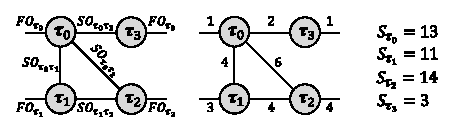
\includegraphics{figure_03_a}
				\caption*{beliebiges Netzwerk mit angegebenen free/sharing orders}
			\end{figure}
		\end{frame}

		\begin{frame}{Beispielkontraktionen und Berechnung von MC/MS}
			\begin{figure}
				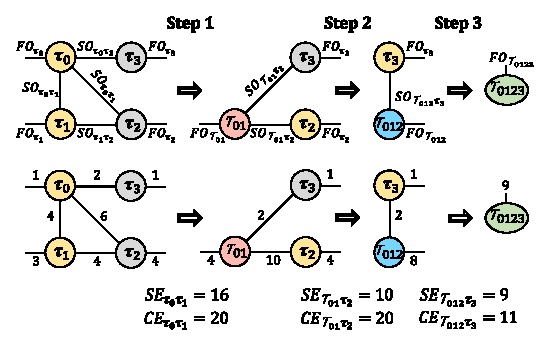
\includegraphics{figure_03_b}
				\caption*{beliebige Kontraktion mit Angabe des jeweiligen SE und CE}
			\end{figure}
		\end{frame}

		\begin{frame}{Beispielkontraktionen und Berechnung von MC/MS}
			\begin{figure}
				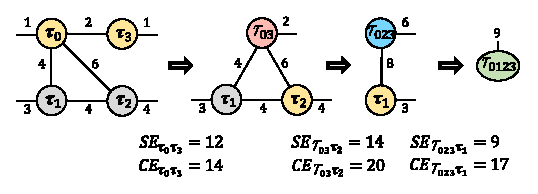
\includegraphics{figure_03_c}
				\caption*{Kontraktion mit bestmöglichem MS}
			\end{figure}
		\end{frame}

		\begin{frame}{Beispielkontraktionen und Berechnung von MC/MS}
			\begin{figure}
				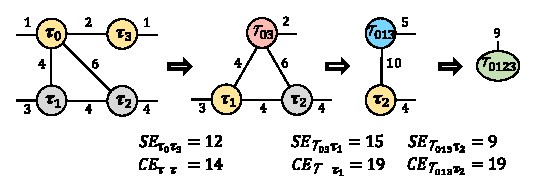
\includegraphics{figure_03_d}
				\caption*{Kontraktion mit bestmöglichem MC}
			\end{figure}
		\end{frame}

		\begin{frame}{Beispielkontraktionen und Berechnung von MC/MS}
			\begin{align*}
				sq_{MS} &= (((\bm{\tau}_{0} \bm{\tau}_{3}) \bm{\tau}_{2}) \bm{\tau}_{1}) \\
				sq_{MC} &= (((\bm{\tau}_{0} \bm{\tau}_{3}) \bm{\tau}_{1}) \bm{\tau}_{2})
			\end{align*}
			\begin{equation*}
				\rightarrow sq_{MS} \neq sq_{MC}
			\end{equation*}
			\begin{itemize}
				\item die Kontraktionsreihenfolgen für den kleinsten Speicher- bzw. Rechenaufwand sind nicht zwangsläufig identisch
				\item es muss entschieden werden, was optimiert werden soll
			\end{itemize}
		\end{frame}


	\section{$Set_v$ und $Split_v$}

		\begin{frame}{$Set_v$ und $Split_v$}
			\begin{itemize}
				\item $Set_v$ ist die Menge aller möglichen Tensoren, welche aus $v$ ursprünglichen Tensoren kontrahiert wurden in einem Netzwerk mit $V$ Tensoren
				\item für $V = 3$ ist $Set_2 = \{\bm{T}_{01}, \bm{T_}{02}, \bm{T}_{12} \}$ und $Set_3 = \{\bm{T}_{012} \}$
			\end{itemize}
		\end{frame}

		\begin{frame}{$Set_v$ und $Split_v$}
			\begin{itemize}
				\item jeder Tensor aus $Set_v$ kann auf $Split_v$ verschiedene Arten in einem Schritt aus zwei verschiedenen Teiltensoren kontrahiert werden
				\item der Tensor $\bm{T}_{012} \in Set_3$ kann kontrahiert werden aus $\{\bm{\tau}_0, \bm{T}_{02} \}$, $\{\bm{\tau}_{1}, \bm{T}_{02} \}$ oder $\{\bm{\tau}_{2}, \bm{T}_{01} \}$ $\rightarrow Split_3 = 3$
			\end{itemize}
			\begin{align*}
				Split_v &= \begin{cases}
					\sum^{\lfloor v/2 \rfloor}_{k=1} \binom{v}{k} &\text{falls v ungerade} \\
					\sum^{\lfloor v/2 \rfloor}_{k=1} \binom{v}{k} + \frac{\binom{v}{v/2}}{2} & \text{falls v gerade}
				\end{cases} \\
				&= \frac{2^v - 2}{2} = \mathcal{O}(2^v)
			\end{align*}
		\end{frame}
	
	
		\section{Verwendete Datenstrukturen}
		\subsection{Adjazenzmatrix für Sharing-Orders}

			\begin{frame}{Aufbau der verwendeten Datenstruktur}
				\begin{itemize}
					\item das Tensorennetzerk wird als ein ungerichteter Graph angesehen
					\item es wird eine Adjazenzmatrix verwendet, um die Sharing-Orders zu speichern und auf sie zuzugreifen
					\item die Matrix ist hierbei nicht symmetrisch, 
					sondern es gilt $SO_{\bm{\tau}_i \bm{\tau}_j} = E_{\bm{\tau}_i \bm{\tau}_j} + E_{\bm{\tau}_j \bm{\tau}_i}$, wobei $E_{\bm{\tau}_a \bm{\tau}_b}$ der jeweilige Eintrag in der Zeile von $\bm{\tau}_a$ und Spalte von $\bm{\tau}_b$ ist und $E_{\bm{\tau}_a \bm{\tau}_b} \in \mathbb{N}_0$.
				\end{itemize}
				\begin{figure}
					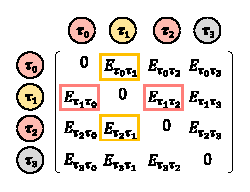
\includegraphics{figure_05_a}
				\end{figure}
			\end{frame}

			\begin{frame}{Beispiel einer Adjazenzmatrix}
				\begin{columns}
					\column{.5\textwidth}
					\begin{figure}
						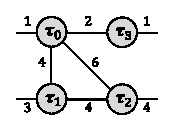
\includegraphics[scale=1.7]{figure_03_a_mid}
						\caption*{Tensornetzwerk mit eingetragenen Sharing-Orders}
					\end{figure}
					\column{.5\textwidth}
					\begin{figure}
						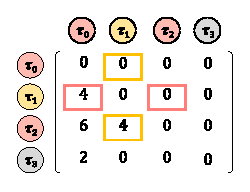
\includegraphics[scale=1.3]{figure_05_c}
						\caption*{eine mögliche zum Netzerk gehörende Adjazenzmatrix}
					\end{figure}
				\end{columns}
			\end{frame}

			\begin{frame}{Zeilenvektoren von zusammengesetzten Tensoren}
				\begin{itemize}
					\item \textit{zur Erinnerung:} $SO_{\bm{T}_I \bm{T}_J} = \sum_m \log_k N^m_{\bm{T}_I \bm{T}_J}$
					\item somit ist beispielsweise $SO_{\bm{\tau}_1 \bm{T}_{02}} = SO_{\bm{\tau}_1 \bm{\tau}_0} + SO_{\bm{\tau}_1 \bm{\tau}_2}$
				\end{itemize} \pause

				\begin{figure}
					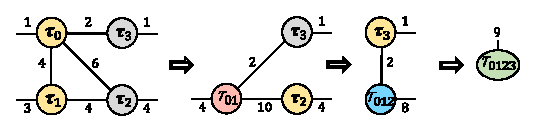
\includegraphics{figure_03_b_low}
				\end{figure}
			\end{frame}

			\begin{frame}{Zeilenvektoren von zusammengesetzten Tensoren}
				\begin{figure}
					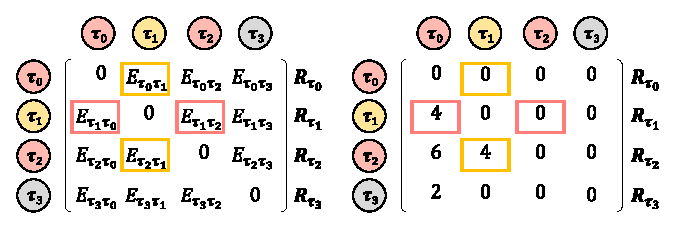
\includegraphics[scale=.9]{figure_05_a_c}
				\end{figure} \pause
				\begin{figure}
					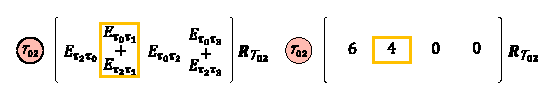
\includegraphics[scale=1.1]{figure_05_b_d}
				\end{figure} \pause
				\begin{equation*}
					SO_{\bm{T}_{02} \bm{\tau}_1} = R_{\bm{T}_{02}}[1] + R_{\bm{\tau}_1}[0] + R_{\bm{\tau}_1}[2]
				\end{equation*}
			\end{frame}

			\begin{frame}{Zeilenvektoren von zusammengesetzten Tensoren}
				\begin{itemize}
					\item die Zeilenvektoren möglicher Tensoren werden gespeichert
					\item dies ermöglicht eine effiziente Berechnung von Zeilenvektoren größerer Tensoren und somit deren Shared-Orders
				\end{itemize}
				\begin{equation*}
					R_{\bm{T}_I} = R_{\bm{T}_J} + R_{\bm{T}_K}, J \cup K = I \wedge J \cap K = \emptyset
				\end{equation*} \pause
				\begin{itemize}
					\item auch der $SE$ eines Tensors wird mit Hilfe eines beliebigen Split-Cases berechnet und gespeichert
				\end{itemize}
				\begin{equation*}
					SE_{\bm{T}_I \bm{T}_J} = S_{\bm{T}_{I}} + S_{\bm{T}_{J}} - 2SO_{\bm{T}_I \bm{T}_J}
				\end{equation*}
			\end{frame}

			\subsection{Adjazenzmatrix zum Finden von Outer-Products}
			\begin{frame}{Finden von Outer-Products}
				\begin{itemize}
					\item das Kontrahieren zweier Tensoren ohne Sharing-Order ist ein Outer-Product
					\item diese Outer-Products müssen nicht beachtet werden, da es immer eine Kontraktionssequenz ohne Outer-Products gibt, welche den kleinsten $MC$ bzw. $MS$ besitzt\cite{outerProduct}
					\item es wird eine ähnliche Datensturktur wie zuvor verwendet, um Outer-Products zu finden
				\end{itemize} \pause
				\begin{equation*}
					\rightarrow \text{zu finden sind Tensoren, sodass } SO_{\bm{T}_I \bm{T}_J} = 0
				\end{equation*}
			\end{frame}

			\begin{frame}{Finden von Outer-Products}
				\begin{figure}
					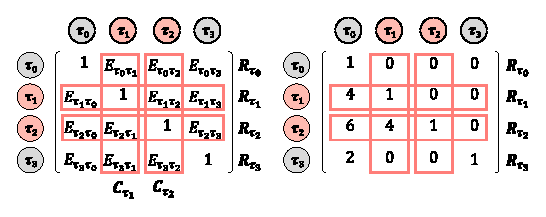
\includegraphics[scale=1.1]{figure_05_e_g}
				\end{figure} \pause
				\begin{figure}
					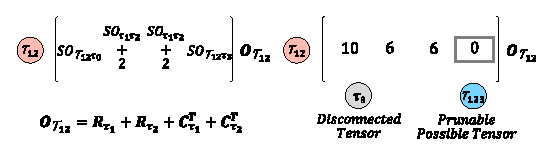
\includegraphics[scale=1.2]{figure_05_f_h}
				\end{figure}
			\end{frame}

			\begin{frame}{Finden von Outer-Products}
				\begin{itemize}
					\item es wird ein Zeilenvektor $O_{\bm{T}_I}$ berechnet
					\item an den Spalten (und den dazugehörigen Tensoren), welche gleich $0$ sind, sind die Tensoren ablesbar, welche keine Sharing-Orders mit $\bm{T}_I$ haben
					\item diese können im späteren Algorithmus ignoriert werden \pause
					\item die Diagonale der verwendeten Matrix ist $1$, damit Tensoren, welche sich schon in der Menge $I$ aus $\bm{T}_I$ befinden, grundsätzlich einen Wert größer $0$ in $O_{\bm{T}_I}$ haben
				\end{itemize}
			\end{frame}
	

		\section{Algorithmus}
		\subsection{Parallelisierung}

			\begin{frame}{Parallelisierung}
				\begin{itemize}
					\item die Berechnungen für die möglichen Tensoren aus $Set_v$ lassen sich einfach auf mehrere Threads aufteilen
					\item für Tensoren innerhalb eines $Set_v$ gibt es keine voneinander abhängigen Berechnungen
				\end{itemize}
				\begin{figure}
					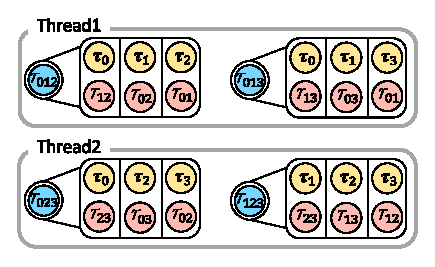
\includegraphics{figure_07}
				\end{figure}
			\end{frame}

			\begin{frame}{Parallelisierung}
				\begin{itemize}
					\item in der \textit{vanilla search} gibt es keine Speicherkonflikte, denn es werden nur für die Tensoren spezifische Werte ausgerechnet: Speicherkosten, Zeilenvektoren, LME \pause
					\item in der \textit{Suche mit Weglassen von Outer-Products} werden zusätzlich noch die Outer-Product-Vektoren der Tensoren berechnet, was ebenfalls tensorenspezifische Werte sind
					\item unterschiedliche Threads mit unterschiedlichen Tensoren finden möglicherweise einen gleichen Tensor, welcher nicht beachtet werden muss
					\item somit wird gleichzeitig auf das gleiche $P_{\bm{T}_I}$ geschrieben, jedoch immer mit demselben Datum
				\end{itemize} \pause
				$\rightarrow$ keine Speicherkonflikte
			\end{frame}

		
		\section{Experimentelle Resultate}
		\subsection{Vanilla Search}

		\begin{frame}{Experimentelle Resultate Vanilla Search}
			\begin{itemize}
				\item die für das Testen verwendeten Tensornetzwerke sind komplett vernetzt
			\end{itemize}
			\begin{figure}
				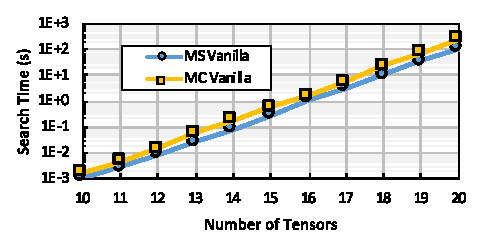
\includegraphics{figure_08}
			\end{figure} \pause
			$\rightarrow$ MS Vanilla ist schneller als MC Vanilla
		\end{frame}

		\begin{frame}{Experimentelle Resultate Vanilla Search}
			\begin{itemize}
				\item ein zusätzlicher Tensor führt ungefähr zu einer Verdreifachung der Suchzeit
			\end{itemize}
			\begin{figure}
				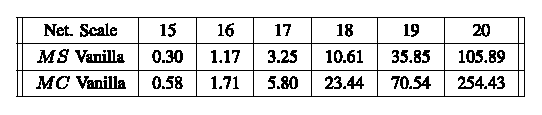
\includegraphics{table_02}
			\end{figure}
			\begin{equation*}
				Split_{total} = \sum^V_{v=1} \binom{V}{v} \cdot Split_v = \sum^v_{v=1} \binom{V}{v} \cdot \mathcal{O} \left(2^V \right) = \mathcal{O} \left(3^V \right)
			\end{equation*}
		\end{frame}

	\subsection{Parallelisierung}

		\begin{frame}{Experimentelle Resultate Parallelisierung}
			\begin{itemize}
				\item getestet wurde mit einem Tensornetzwerk in Form eines Binärbaumes mit 19 Tensoren und 25\% extra Kanten
			\end{itemize}
			\begin{figure}
				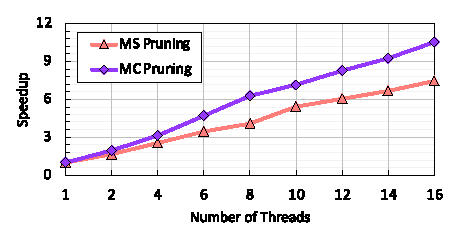
\includegraphics{figure_13}
			\end{figure} \pause
			\begin{itemize}
				\item MC ergibt eine größere Beschleunigung als MS
				\item bei einer größeren Anzahl an Threads wird die Geschwindigkeitszunahme kleiner
			\end{itemize}
		\end{frame}
	
	
	\begin{frame}[allowframebreaks]{Bibliography}
		\bibliography{../bibliography/bibliography.bib}
		\bibliographystyle{unsrt}
	\end{frame}
	
\end{document}
